\documentclass[12pt, a4paper]{article}

\usepackage{lastpage}
\usepackage{mathtools}
\usepackage{xltxtra}
\usepackage{libertine}
\usepackage{amsmath}
\usepackage{amsthm}
\usepackage{amsfonts}
\usepackage{amssymb}
\usepackage{enumitem}
\usepackage{xcolor}
\usepackage[left=1.5cm, right=1.5cm, top=2cm, bottom=2cm, bindingoffset=0cm, headheight=15pt]{geometry}
\usepackage{fancyhdr}
\usepackage[russian]{babel}
% \usepackage[utf8]{inputenc}
\usepackage{catchfilebetweentags}
\usepackage{accents}
\usepackage{calc}
\usepackage{etoolbox}
\usepackage{mathrsfs}
\usepackage{wrapfig}

\providetoggle{useproofs}
\settoggle{useproofs}{false}

\pagestyle{fancy}
\lfoot{M3137y2019}
\rhead{\thepage\ из \pageref{LastPage}}

\newcommand{\R}{\mathbb{R}}
\newcommand{\Q}{\mathbb{Q}}
\newcommand{\C}{\mathbb{C}}
\newcommand{\Z}{\mathbb{Z}}
\newcommand{\B}{\mathbb{B}}
\newcommand{\N}{\mathbb{N}}

\newcommand{\const}{\text{const}}

\newcommand{\teormin}{\textcolor{red}{!}\ }

\DeclareMathOperator*{\xor}{\oplus}
\DeclareMathOperator*{\equ}{\sim}
\DeclareMathOperator{\Ln}{\text{Ln}}
\DeclareMathOperator{\sign}{\text{sign}}
\DeclareMathOperator{\Sym}{\text{Sym}}
\DeclareMathOperator{\Asym}{\text{Asym}}
% \DeclareMathOperator{\sh}{\text{sh}}
% \DeclareMathOperator{\tg}{\text{tg}}
% \DeclareMathOperator{\arctg}{\text{arctg}}
% \DeclareMathOperator{\ch}{\text{ch}}

\DeclarePairedDelimiter{\ceil}{\lceil}{\rceil}
\DeclarePairedDelimiter{\abs}{\left\lvert}{\right\rvert}

\setmainfont{Linux Libertine}

\theoremstyle{plain}
\newtheorem{axiom}{Аксиома}
\newtheorem{lemma}{Лемма}

\theoremstyle{remark}
\newtheorem*{remark}{Примечание}
\newtheorem*{exercise}{Упражнение}
\newtheorem*{consequence}{Следствие}
\newtheorem*{example}{Пример}
\newtheorem*{observation}{Наблюдение}

\theoremstyle{definition}
\newtheorem{theorem}{Теорема}
\newtheorem*{definition}{Определение}
\newtheorem*{obozn}{Обозначение}

\setlength{\parindent}{0pt}

\newcommand{\dbltilde}[1]{\accentset{\approx}{#1}}
\newcommand{\intt}{\int\!}

% magical thing that fixes paragraphs
\makeatletter
\patchcmd{\CatchFBT@Fin@l}{\endlinechar\m@ne}{}
  {}{\typeout{Unsuccessful patch!}}
\makeatother

\newcommand{\get}[2]{
    \ExecuteMetaData[#1]{#2}
}

\newcommand{\getproof}[2]{
    \iftoggle{useproofs}{\ExecuteMetaData[#1]{#2proof}}{}
}

\newcommand{\getwithproof}[2]{
    \get{#1}{#2}
    \getproof{#1}{#2}
}

\newcommand{\import}[3]{
    \subsection{#1}
    \getwithproof{#2}{#3}
}

\newcommand{\given}[1]{
    Дано выше. (\ref{#1}, стр. \pageref{#1})
}

\renewcommand{\ker}{\text{Ker }}
\newcommand{\im}{\text{Im }}
\newcommand{\grad}{\text{grad}}

\lhead{Математический анализ}
\cfoot{}
\rfoot{21.12.2020}

\begin{document}

\begin{corollary}[из 5 свойства меры Лебега]
    \(\forall A\in \mathfrak{M}^m\ \ \exists B,C\) --- борелевские:
    \[B\subset A\subset C \quad \lambda(C\setminus A) = 0, \lambda(A\setminus B) = 0\]
\end{corollary}
\begin{proof}
    \[C: = \bigcap_{n = 1}^{+\infty} G_{\frac{1}{n}} \quad B \subset \bigcup_{n = 1}^{+\infty} F_{\frac{1}{n}}\]
\end{proof}
\begin{corollary}
    \(\forall A\in \mathfrak{M}^m \ \ \exists B, \mathcal{N} : B\) --- борелевское, \(\mathcal{N}\in \mathfrak{M}^m, \lambda \mathcal{N} = 0\).

    Тогда \(A = B \cup \mathcal{N}\)
\end{corollary}
\begin{proof}
    \(\exists B\) из следствия 1, \(\mathcal{N} : = A\setminus B\)
\end{proof}

\begin{remark}
    Обозначим \(|X|\) --- мощность множества \(X\).

    \[\forall X \ \ |2^X| > |X|\]
    \[|2^{\R^m}| > \text{континуум}\]
    \[\mathcal{B} \subset 2^{\R^m} \text{ --- борелевская \(\sigma\)-алгебра} \ \ |\mathcal{B}| = \text{континуум}\]
    \[\mathfrak{M}^m > \text{континуум}\]
    \(\mathcal{K}\) --- Канторово множество, тогда \(|\mathcal{K}|=\) континуум, \(\lambda \mathcal{K} = 0\)
    \[\forall D\subset \mathcal{K}\ \ D\in \mathfrak{M}^m, \lambda D = 0 \ \ 2^{\mathcal{K}} \subset \mathfrak{M}^m\]
\end{remark}

\begin{corollary}
    %<*регулярностьмерылебега>
    \(\forall A\in \mathfrak{M}^m\)
    \[\lambda A = \inf_{\substack{G:A\subset G\\ G \text{ --- откр.}}} \lambda(G) = \sup_{\substack{F:F\subset A\\ F \text{ --- замкн.}}} \lambda(F) \stackrel{(*)}{=} \sup_{\substack{K:K\subset A\\ K \text{ --- комп.}}} \lambda(K)\]
    %</регулярностьмерылебега>
\end{corollary}
%<*регулярностьмерылебегаproof>
\begin{proof}
    \((*)\) следует из \(\sigma\)-конечности \(\R^m = \bigcup\limits_{n = 1}^{+\infty} Q(0, n)\), где \(Q(a, R) = \times_{i = 1}^n [a_i - R, a_i + R]\) --- куб с центром в \(a\) и ребром \(R\).

    \(\lambda(A\cap Q(0, n)) \to \lambda A\) по непрерывности снизу, т.к. \(A\cap Q(0, n)\) хорошо аппроксимируется замкнутым множеством.
\end{proof}
%</регулярностьмерылебегаproof>

\begin{definition}
    Свойства из следствия 3 называются \textbf{регулярностью} меры Лебега.
\end{definition}

\section*{Преобразование меры Лебега при сдвигах и линейных отображениях}

\begin{lemma}\itemfix
    \begin{itemize}
        \item \((X', \mathfrak{A}', \mu')\) --- пространство с мерой.
        \item \((X, \mathfrak{A}, \_)\) --- ``заготовка'' пространства с мерой
        \item \(\exists T : X \to X'\) --- биекция; \(\forall A\in \mathfrak{A}\ \ TA\in \mathfrak{A}'\) и \(T\emptyset = \emptyset\)
    \end{itemize}

    Положим \(\mu A = \mu'(TA)\). Тогда \(\mu\) --- мера.
\end{lemma}
\begin{proof}
    Проверим счётную аддитивность \(\mu\) : \(A = \bigsqcup A_i\)
    \[\mu A = \mu'(TA) = \mu'\left(\bigsqcup TA_i\right) = \sum \mu'(TA_i) = \sum \mu A_i\]
\end{proof}

\begin{lemma}\itemfix
    %<*непрерывноеотображениеизмеримость>
    \label{непр изм}
    \begin{itemize}
        \item \(T : \R^m \to \R^n\) --- непр.
        \item \(\forall E\in \mathfrak{M}^m : \lambda E = 0\) выполняется \(\lambda TE = 0\)
    \end{itemize}
    Тогда \(\forall A\in \mathfrak{M}^m \ \ TA\in \mathfrak{M}^m\)
    %</непрерывноеотображениеизмеримость>
\end{lemma}
%<*непрерывноеотображениеизмеримостьproof>
\begin{proof}
    \[A = \bigcup_{j = 1}^{+\infty} K_j\cup \mathcal{N}\]
    , где \(K_j\) --- компакт, \(\lambda \mathcal{N} = 0\)
    \[TA = \bigcup_{j = 1}^{+\infty} TK_j \cup T\mathcal{N}\]
    \(TK_j\) компакт как образ компакта при непрерывном отображении. \(\Rightarrow TA\) измеримо.
\end{proof}
%</непрерывноеотображениеизмеримостьproof>

\begin{example}[Канторова лестница]
    \begin{figure}[h]
        \centering
        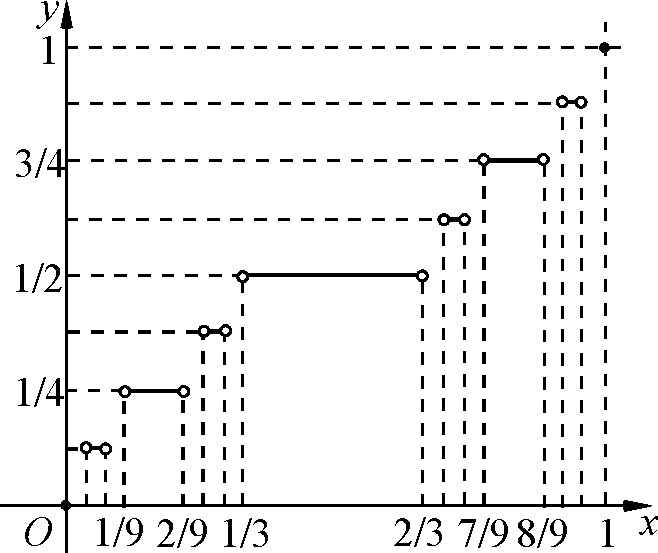
\includegraphics[scale=0.5]{images/cantor_ladder.png}
    \end{figure}
    \[\Delta = [0, 1]\]
    \[\Delta_0 = \left[0, \frac{1}{3}\right] \quad \Delta_1 = \left[\frac{2}{3}, 1\right]\]
    \[\Delta_{00} = \left[0, \frac{1}{9}\right] \quad \Delta_{01} = \left[\frac{2}{9}, \frac{1}{3}\right], \Delta_{10} = \dots, \Delta_{11} = \dots \]
    \begin{align*}
        \mathcal{K}_0 & = \Delta                                                                                               \\
        \mathcal{K}_1 & = \Delta_0\cup \Delta_1                                                                                \\
        \mathcal{K}_2 & = \Delta_{00}\cup \Delta_{01}\cup \Delta_{10}\cup \Delta_{11}                                          \\
                      & \vdots                                                                                                 \\
        \mathcal{K}_n & = \bigcup_{\varepsilon_1 \dots \varepsilon_n \in \{0, 1\} } \Delta_{\varepsilon_1 \dots \varepsilon_n}
    \end{align*}
    \[\mathcal{K} : = \bigcap \mathcal{K}_n\]
    \[f(x) = \begin{cases}
            \frac{1}{2} & , x\in \Delta\setminus \mathcal{K}_1   \\
            \frac{1}{4} & , x\in \Delta_0\setminus \mathcal{K}_2 \\
            \frac{3}{4} & , x\in \Delta_1\setminus \mathcal{K}_2 \\
            \vdots                                               \\
            \sup f(t)   & , t \leq x, t\not\in \mathcal{K}
        \end{cases}\]

    \(f([0, 1]\setminus \mathcal{K}\) --- счётное = множество двоично-рациональных чисел из \([0, 1]\)

    \(\lambda f([0, 1]\setminus \mathcal{K}) = 0\)

    \(\lambda f(\mathcal{K}) = 1\), т.к. \(\forall y\in [0, 1] \ \ \exists x : f(x) = y\), при этом \(f\) непрерывна, т.к. она --- сюръекция.

    Тогда пусть \(E\subset [0, 1]\not\in \mathfrak{M}^m\) : \(f^{ - 1}(E)\) --- подмножество \(\mathcal{K}\) и промежутки --- прообразы двоично рациональных точек \(\in E\), при этом это множество измеримо, т.к. \(\lambda \mathcal{K} = 0\)

    Ещё наблюдение: \(x\not\in \mathcal{K} \Rightarrow f\) --- дифференцируема в \(x\) и \(f' = 0\)
\end{example}

\begin{theorem}\itemfix
    %<*гладкоеотображениеизмеримость>
    \begin{itemize}
        \item \(O\subset \R^m\) открыто
        \item \(\Phi: O \to \R^n\)
        \item \(\Phi\in C^1(O)\)
    \end{itemize}
    Тогда \(\forall A\in O : A \in \mathfrak{M}^m \ \ \Phi(A)\in \mathfrak{M}^m\), т.е. образ измеримого множества измерим.
    %</гладкоеотображениеизмеримость>
\end{theorem}
%<*гладкоеотображениеизмеримостьproof>
\begin{proof}
    Достаточно проверить свойства \(\lambda E = 0 \Rightarrow \lambda \Phi(E) = 0\), т.к. если оно выполняется, то работает предыдущая лемма \ref{непр изм}
    \[\lambda E = 0 \Leftrightarrow \forall \varepsilon > 0 \ \ \exists \text{ шары } B_i : E \subset \bigcup_{i=1}^{+\infty} B_i \quad \lambda B_i < \varepsilon\]
    \( \Rightarrow \) из теоремы о Лебеговском продолжении меры.

    \( \Leftarrow \) по полноте меры Лебега.

    \begin{enumerate}
        \item \(E\subset P \subset \overline P \subset O, \lambda E = 0\)
              \[L : = \max_{x\in \overline P} | |\Phi'(x)| |\]
              Тогда
              \[\forall x, y\in P \ \ |\Phi(x) - \Phi(y)| \leq L|x - y|\]
              --- неравенство Лагранжа.
              \[\Phi(B(x_0, r)) \subset B(\Phi(x_0), Lr) \subset Q(\Phi(x_0), Lr)\]
              \[B_i := B(x_i, r_i), y_i := \Phi(x_i)\]
              \[E\subset \bigcup B_i \ \ \sum \lambda B_i < \varepsilon \Rightarrow\]
              \[\Phi(E) \subset \bigcup \Phi(B_i) \subset \bigcup B(y_i, Lr) \subset \bigcup Q(y_i, Lr)\]
              \[\sum \lambda \Phi(B_i) < \sum \lambda Q(y_i, Lr_i)  = \sum (2Lr_i)^m = (2L)^m \sum r_i^m\]
              Было \(\sum (2r_i)^m < \varepsilon (\sqrt{m})^m\), стало \(\sum \lambda \Phi(B_i) < L^m \sum (2r_i)^m < \varepsilon (\sqrt{m} L)^m\)
        \item Рассмотрим произвольный случай, то есть \(E\subset O\)

              \(O = \bigsqcup Q_i\), где \(Q_i\) --- кубические ячейки, \(Q_i \subset \overline Q_i \subset O\)

              \(E = \bigsqcup (E\cap Q_i)\), \(\lambda(E\cap Q_i) = 0\). Тогда по пункту 1 \(\lambda(\Phi(E\cap Q_i)) = 0\)
              \[\Phi(E) = \bigcup \Phi(E\cap Q_i) \Rightarrow \lambda \Phi(E) = 0\]
    \end{enumerate}
\end{proof}
%</гладкоеотображениеизмеримостьproof>

%<*инвариантностьмерылебега>
\begin{corollary}
    \(\lambda\) --- инвариантно относительно сдвигов в \(\R^m\) (и \(\mathfrak{M}^m\) тоже инвариантно), т.е. \(\forall a\in\R^m\):
    \begin{align}
        \forall A\in \mathfrak{M}^m & \quad A + a\in \mathfrak{M}^m \label{сдивг измерим}              \\
                                    & \quad \text{ и } \lambda A = \lambda (A + a) \label{мера сдвига}
    \end{align}
\end{corollary}
%</инвариантностьмерылебега>

%<*инвариантностьмерылебегаproof>
\begin{proof}
    \[\Phi : x \mapsto x + a, \Phi\in C^1(\R^m)\]
    Отсюда следует \eqref{сдивг измерим}.

    \eqref{мера сдвига} следует из пункта 5 теоремы о лебеговском продолжении.

    \[A \subset \bigcup P_k \Leftrightarrow A + a \subset \bigcup (P_k + a)\]
    Для ячеек \(\lambda P_k = \lambda(P_k + a)\)

    Таким образом:
    \[\lambda A = \inf \left( \sum \lambda P_k \right) = \inf \left( \sum \lambda (P_k + a) \right) = \lambda (A + a)\]
\end{proof}
%</инвариантностьмерылебегаproof>

\begin{theorem}
    %<*инвариантныемеры>

    \label{инвариантные меры}

    \(\mu\) --- мера на \(\mathfrak{M}^m\):
    \begin{enumerate}
        \item \(\mu\) --- инвариантно относительно сдвигов:
              \[\forall a\in\R^m \ \ \forall E\in \mathfrak{M}^m \ \ \mu(E + a) = \mu E\]
        \item Для любого ограниченного \(E\in \mathfrak{M}^m \ \ \mu(E) < +\infty\)
    \end{enumerate}
    Тогда \(\exists k\in [0, +\infty) : \mu = k\cdot \lambda\), \textit{(где \(\lambda\) --- мера Лебега)} т.е.:
    \[\forall E \ \ \mu E = k \cdot \lambda E\]
    и пусть \(0\cdot \infty = 0\) в данном контексте.
    %</инвариантныемеры>
\end{theorem}
%<*инвариантныемерыproof>
\begin{proof}
    Нет и не будет.

    Общая идея: Как мера \(\mu\) задается на рациональных ячейках?

    В \(\R^2\) \(Q_1\) --- единичная квадратная ячейка, \(\mu Q_1 = v\)

    \(Q_2\) --- ячейка \(2 \times 2\), \(\mu Q_2 = 4v\). Аналогично \(\mu Q_n = n^2 v, \mu Q_{\frac{1}{n}} = \frac{1}{n^2}v\)

    Тогда \(k = v\) и \(\mu\) пропорционально \(\lambda\).
\end{proof}
%</инвариантныемерыproof>

\begin{remark}
    \(\mu A = \lambda_1 A\), если \(\exists y_0 : A\subset \{(x, y_0), x\in \R\} \) --- афинное одномерное подпространство, пересекающее ось \(y\) в точке \(y_0\).

    Эта мера --- 1-Хаусдорфа в \(\R^2\).
\end{remark}

\begin{theorem}[инвариантность меры лебега относительно линейного ортогонального преобразования]\itemfix
    %<*инвариантностьмерылебегаотносительнолинейногоортогональногопреобразования>
    \begin{itemize}
        \item \(T: \R^m \to \R^m\) ортогонально, т.е. сохраняет длины векторов.
    \end{itemize}
    Тогда \(\forall A\in \mathfrak{M}^m\):
    \begin{enumerate}
        \item \(TA\in \mathfrak{M}^m\)
        \item \(\lambda(TA) = \lambda A\)
    \end{enumerate}
    %</инвариантностьмерылебегаотносительнолинейногоортогональногопреобразования>
\end{theorem}
%<*инвариантностьмерылебегаотносительнолинейногоортогональногопреобразованияproof>
\begin{proof}\itemfix
    \begin{enumerate}
        \item \(T\in C^1\), поэтому измеримость сохраняется.
        \item \(\mu A: = \lambda(TA)\)

              \(\mu \) --- мера на \(\mathfrak{M}^m\) по лемме о заготовке пространства, т.к. \(T\) биективно, при этом \(\mu\) инвариантно относительно сдвигов:
              \[\mu(A + a) = \lambda(T(A + a)) = \lambda(TA + Ta) = \lambda(TA) = \mu A\]
              \(A\) ограничено \( \Rightarrow TA\) ограничено \( \Rightarrow \mu A < +\infty\)

              По теореме \ref{инвариантные меры} \(\lambda(TA) = k\cdot \lambda (A)\). Какое у нас \(k\)?

              Возьмём шар \(B\). \(TB\) --- шар того же радиуса, т.е. \(TB\) --- сдвинутый \(B\), т.е. \(TB = B + x_0\).
              \[\mu B = \lambda(TB) = \lambda(B + x_0) = \lambda B \Rightarrow k = 1\]
    \end{enumerate}
\end{proof}
%</инвариантностьмерылебегаотносительнолинейногоортогональногопреобразованияproof>

\begin{corollary}
    \(\lambda(\text{прямоугольный параллелепипед})\) = произведение сторон.
\end{corollary}
\begin{corollary}
    Любое собств. линейное подпространство в \(\R^m\) имеет меру \(0\)
\end{corollary}
\begin{proof}
    Достаточно доказать, что \(\lambda \{x : x_m = 0\} = 0\)
    \[L = \{x : x_m = 0\} \simeq \R^{m - 1} = \bigsqcup \underbrace{Q_i}_{\text{единичные кубы}}\]
    \[L\subset \bigsqcup Q_i \times \left[ -\frac{\varepsilon}{2^i}, \frac{\varepsilon}{2^i} \right)\]
    \[\lambda\left(Q_i \times \left[ -\frac{\varepsilon}{2^i}, \frac{\varepsilon}{2^i} \right)\right) = \frac{2\varepsilon}{2^i} \]
\end{proof}

\end{document}